\documentclass[11pt,a4paper]{article} 
\usepackage[portuges]{babel}
\usepackage[utf8]{inputenc}
\usepackage{graphicx}
\usepackage{listings}
%\renewcommand{\lstlistingname}{Algoritmo} 
\usepackage{amsthm}
\usepackage{booktabs}
\usepackage{amsfonts}
\usepackage{subcaption}
\newtheorem{lema}{Lema}
\newtheorem{corolario}{Corolario}
\newtheorem{teorema}{Teorema}
\graphicspath{{images//}}

\title{Relatório - Trabalho 2 \\ Algoritmos em grafos}
\author{Ronald A. Kaiser}


\begin{document}
    \maketitle

    \paragraph{}
    Para este trabalho estamos interessados em extrair informações de dois grafos. O primeiro com vértices representando cidades da América do Norte e o segundo, cidades do Brasil\footnote{Nos dois grafos, os pesos das arestas representam distâncias.}. O objetivo é obter suas árvores geradoras mínimas, o menor caminho entre duas cidades específicas e a árvore de menores caminhos a partir de uma dada cidade. 
    
    %===========================================
    \section{Grafo América do Norte}

        \begin{figure}[htb!]
          \begin{center}
              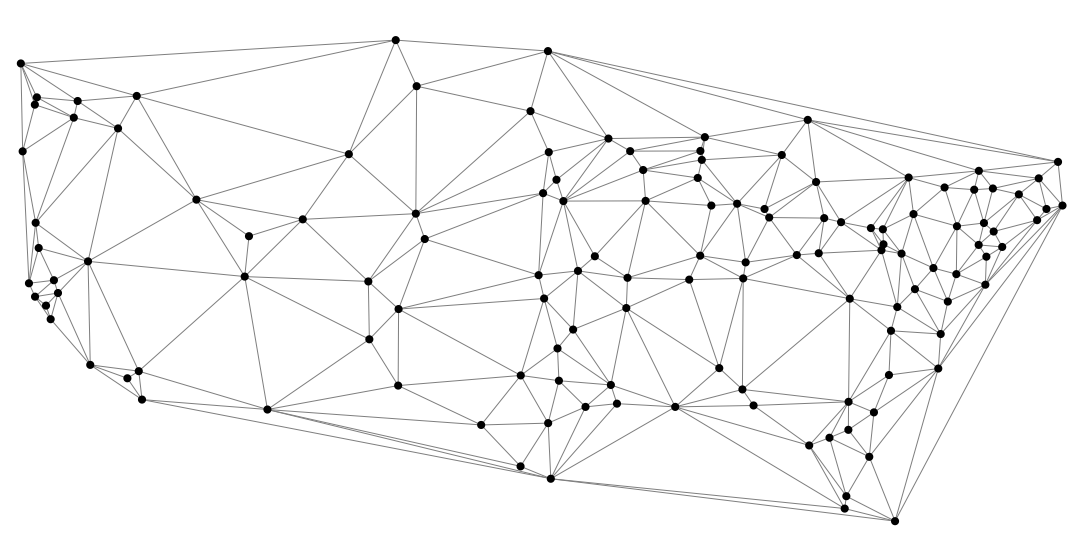
\includegraphics[scale=0.5]{map}
          \end{center}
              \label{fig:map}
              \caption{Grafo das cidades da América do Norte.}
        \end{figure}

        \paragraph{}
        Este grafo possui ${|V|}$ = 128 e ${|E|}$ = 368. Como ${|E|}$ $=$ ${O(3|V|)}$ $=$ ${O(|V|)}$, trata-se de um grafo relativamente esparso. Por este motivo, foi utilizada lista de adjacências para a sua representação interna.

    %-------------------------------------------
    \newpage
        \subsection{Árvore geradora mínima}
        \paragraph{}
        Antes de iniciar o processamento da árvore geradora mínima foi executada uma BFS (poderia ter sido usada uma DFS) no grafo, ignorando-se o peso das arestas, para confirmar de que se tratava de apenas uma componente conexa.

        \paragraph{}
        Após esta confirmação, foi utilizado o algoritmo Kruskal para encontrar uma árvore geradora mínima. O algoritmo de Prim com Heap de Fibonacci também poderia ter sido utilizado, mas seu ganho em termos de tempo não valeria o esforço de implementar a Heap de Fibonacci (mais complicado).

        \begin{figure}[htb!]
          \centering
              \captionsetup{justification=centering}  
              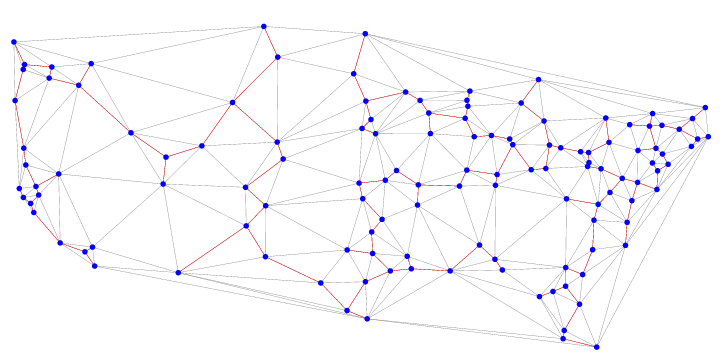
\includegraphics[scale=0.5]{mst_map}
              \label{fig:mstmap}
              \caption{Árvore geradora mínima. Comprimento: 22081.}
        \end{figure}

        \paragraph{}
        Para a implementação do Kruskal, foi utilizada uma heap de mínimo para a ordenação das arestas + Union Find para administrar as componentes do grafo. Foram implementadas 3 versões de Union Find: Quick Find, Quick Union e Quick Union Weighted. Seus tempos de execução estão descritos na tabela a seguir.

        \begin{table}[htb!]
        \centering
            \begin{tabular}{|c|c|}
            \toprule
            Algoritmo                         & Tempo (s)\\
            \midrule
            Kruskal + Quick Find              & 0.003676 \\
            Kruskal + Quick Union             & 0.001749 \\
            Kruskal + Quick Union (Weighted)  & 0.001681 \\
            \bottomrule
            \end{tabular}
            \caption{Execução de Kruskal no grafo América do Norte.}
        \end{table}
        
        \paragraph{}
        Apesar da vantagem do Quick Union (Weighted) não ter ficado clara para este grafo, ela se torna bem evidente quando executamos para o grafo das cidades do Brasil (com mais de 5000 vértices).

    %-------------------------------------------
        \subsection{Menor caminho entre as cidades 93 e 112}
        \paragraph{}
        Para encontrar o menor caminho entre as cidades 93 e 112 foi utilizado o algoritmo de Dijkstra, dado que as arestas do grafo não continham pesos negativos. A cidade 93 serviu de fonte para esta execução. 

        \begin{figure}[htb!]
          \centering
              \captionsetup{justification=centering}  
              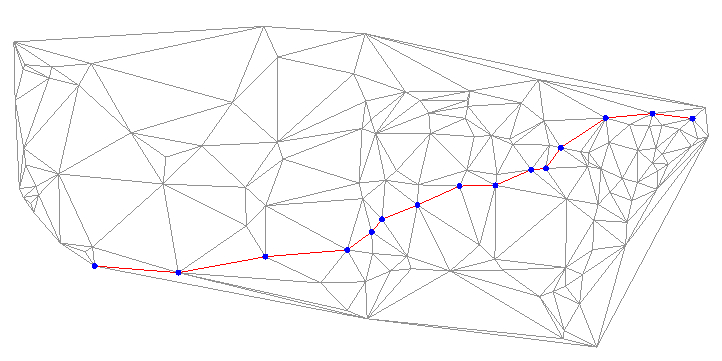
\includegraphics[scale=0.5]{map93-112}
              \label{fig:map93112}
              \caption{Menor caminho entre as cidades 93 e 112. Comprimento: 4737.}
        \end{figure}

    %-------------------------------------------
        \subsection{Árvore de menores caminhos a partir da cidade 104}

        \paragraph{}
        Para encontrar a árvore de menores caminhos foi executado o algoritmo de Dijkstra com fonte na cidade 104. A solução pode ser vista a seguir:

        \begin{figure}[htb!]
          \centering
              \captionsetup{justification=centering}  
              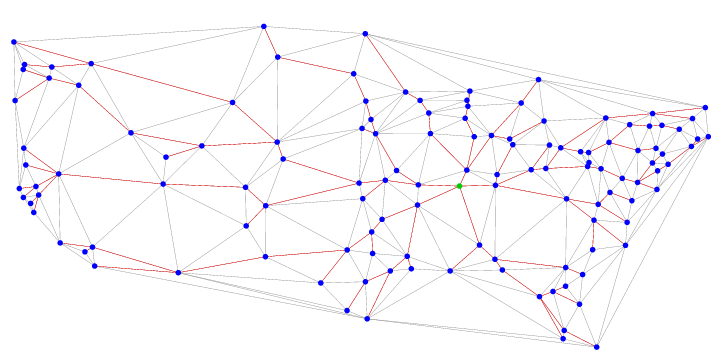
\includegraphics[scale=0.5]{map104}
              \label{fig:map104}
              \caption{Árvore de menores caminhos a partir da cidade 104 (vértice verde). Comprimento: 33314}
        \end{figure}

        \paragraph{}
        Para este fim, duas implementações do Dijkstra foram feitas. Uma utilizando a função de mínimo simples e outra com heap.

        \begin{table}[htb!]
        \centering
            \begin{tabular}{|c|c|}
            \toprule
            Algoritmo                         & Tempo (s)\\
            \midrule
            Dijkstra + simple min             & 0.001562 \\
            Dijkstra + Heap                   & 0.000765 \\
            \bottomrule
            \end{tabular}
            \caption {Execução de Dijkstra para a cidade 104.}
        \end{table}

    %===========================================
    \newpage
    \section{Grafo Brasil}

        \begin{figure}[htb!]
          \centering
              \captionsetup{justification=centering}  
              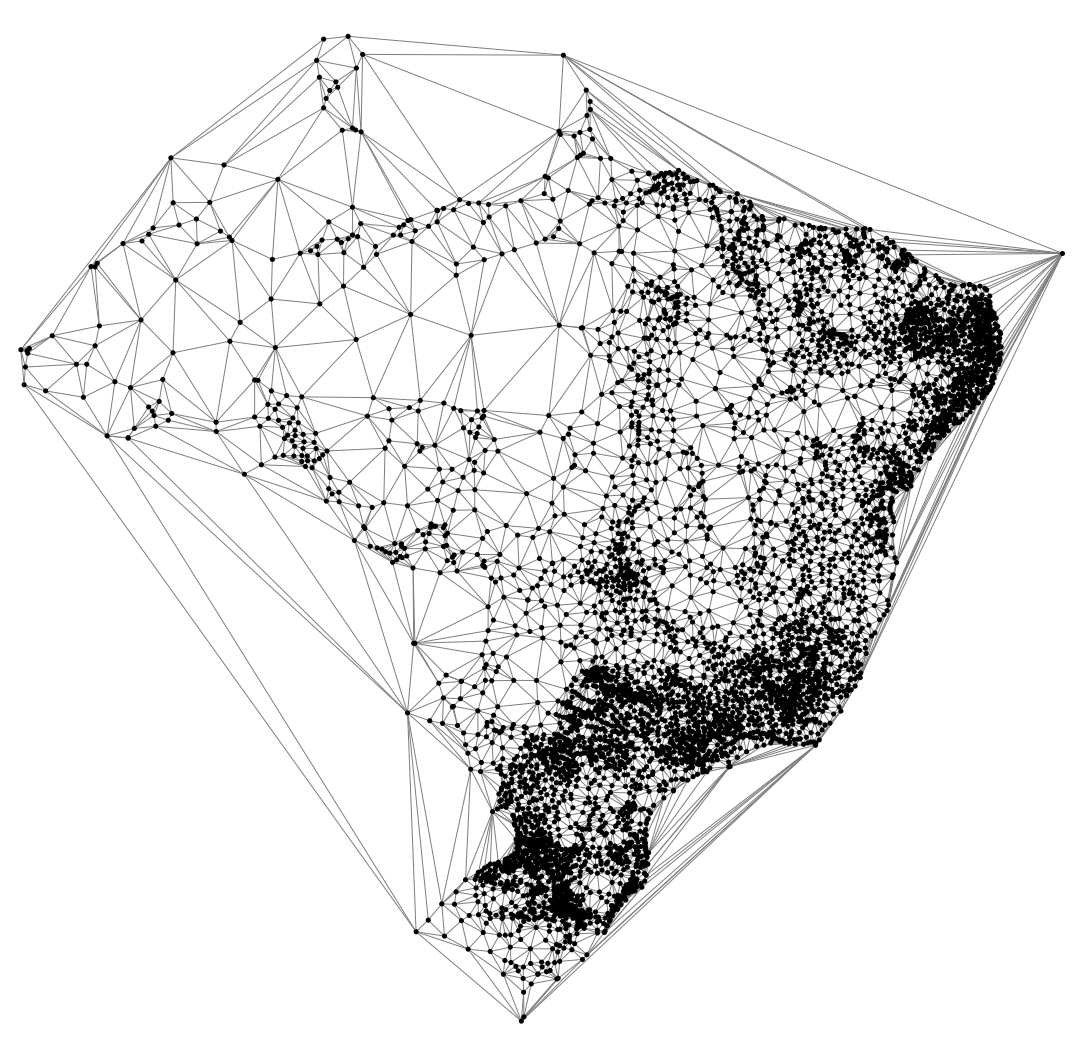
\includegraphics[scale=0.5]{BR}
              \label{fig:BR}
              \caption{Grafo das cidades do Brasil.}
        \end{figure}

        \paragraph{}
        Este grafo possui ${|V|}$ = 5565 e ${|E|}$ = 16680. Assim como no grafo anterior, ${|E|}$ $=$ ${O(3|V|)}$ $=$ ${O(|V|)}$, trata-se de um grafo relativamente esparso. Por este motivo, foi utilizada lista de adjacências para a sua representação interna.

    %-------------------------------------------
        \subsection{Árvore geradora mínima}

        \paragraph{}
        Assim como no grafo anterior, foi executada uma busca para confirmar que o grafo Brasil continha apenas uma componente conexa.
        Para encontrar sua árvore geradora mínima foram utilizados os mesmos algoritmos do grafo anterior. Uma representação da solução pode ser vista a seguir.
        \newpage

        \begin{figure}[htb!]
          \centering
              \captionsetup{justification=centering}  
              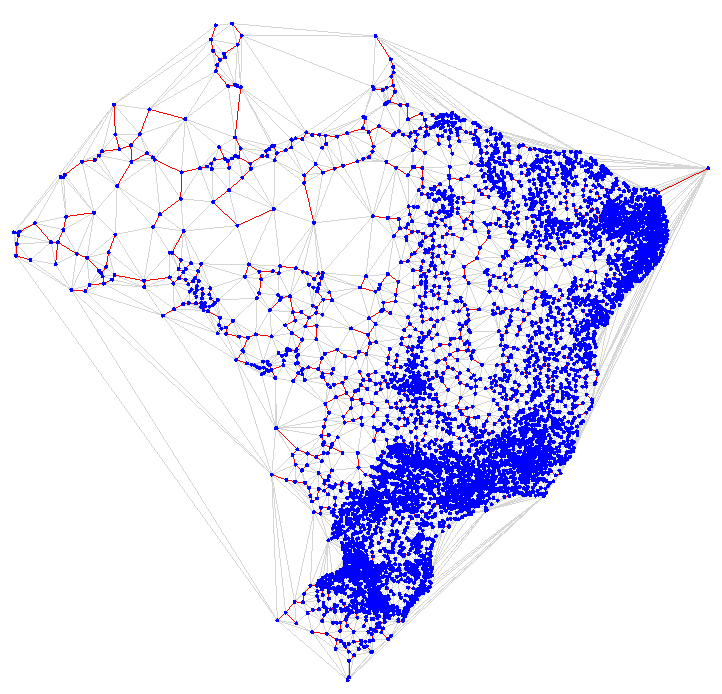
\includegraphics[scale=0.5]{mst_BR}
              \label{fig:mstBR}
              \caption{Árvore geradora mínima. Comprimento: 1040.54151911.}
        \end{figure}

        \begin{table}[htb]
        \centering
            \begin{tabular}{|c|c|}
            \toprule
            Algoritmo                         & Tempo (s)\\
            \midrule
            Kruskal + Quick Find              & 1.296344 \\
            Kruskal + Quick Union             & 0.224946 \\
            Kruskal + Quick Union (Weighted)  & 0.123472 \\
            \bottomrule
            \end{tabular}
            \caption {Execução de Kruskal para o grafo Brasil.}
        \end{table}

        \paragraph{}
        Repare que agora o Quick Union (Weighted) começa a representar uma vantagem no desempenho. Uma implementação com compressão de caminhos provavelmente melhoraria ainda mais o tempo.
        \newpage

    %-------------------------------------------
        \subsection{Menor caminho entre as cidades 1 e 2646}
        \paragraph{}
        Para encontrar o menor caminho entre as cidades 1 e 2646 foi utilizado o algoritmo de Dijkstra com fonte na cidade 2646.  Veja solução a seguir:

        \begin{figure}[htb!]
          \centering
              \captionsetup{justification=centering}  
              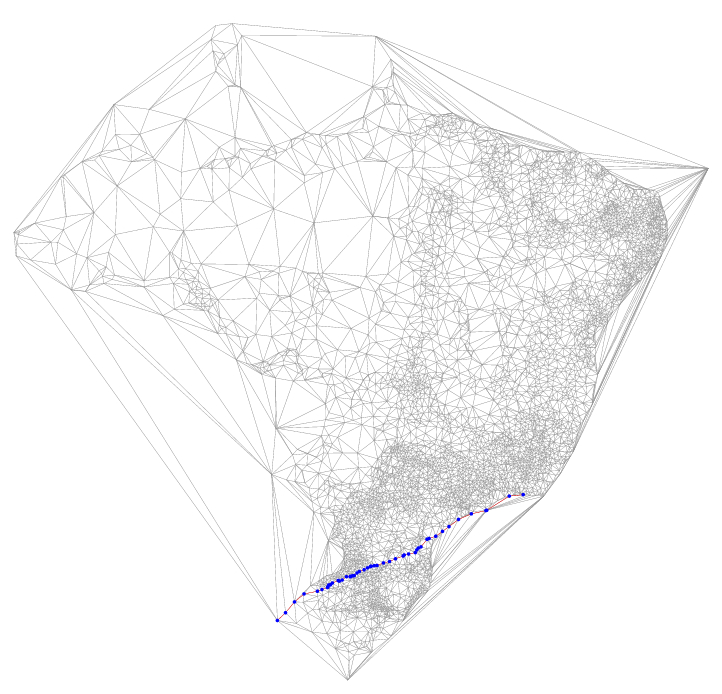
\includegraphics[scale=0.45]{BR1-2646}
              \label{fig:BR12646}
              \caption{Menor caminho entre as cidades 1 e 2646. Comprimento: 16.6558691.}
        \end{figure}

    %-------------------------------------------
        \subsection{Árvore de menores caminhos a partir da cidade 2646}
        \paragraph{}
        Para encontrar a árvore de menores caminhos foi reaproveitado o resultado da execução do Dijkstra com fonte na cidade 2646.

        \paragraph{}
        Neste grafo, a diferença no tempo de execução entre as duas versões do Dijkstra implementadas se torna substancial.

        \begin{figure}[htb!]
          \centering
              \captionsetup{justification=centering}  
              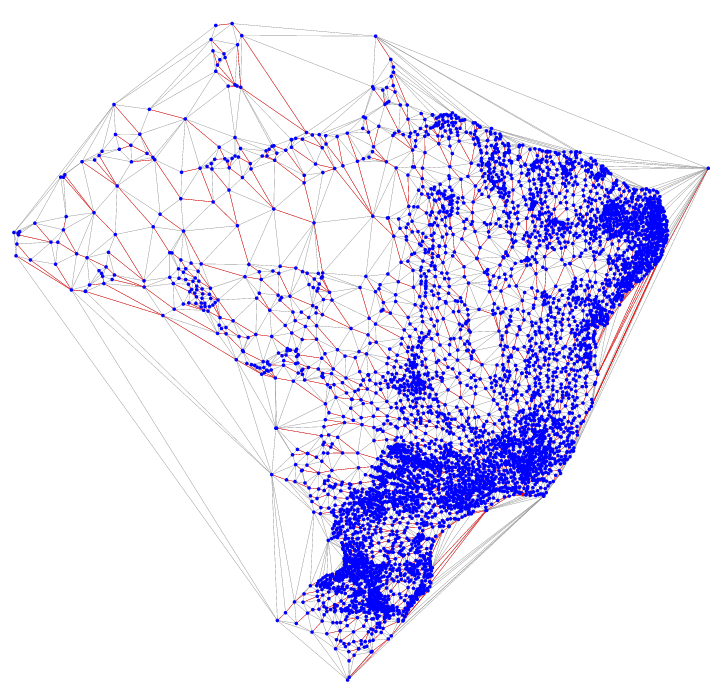
\includegraphics[scale=0.45]{BR2646}
              \label{fig:BR2646}
              \caption{Árvore de menores caminhos a partir da cidade 2646 (vértice vermelho próximo ao Rio de Janeiro). Comprimento: 1715.81175366}
        \end{figure}


        \begin{table}[htb!]
        \centering
            \begin{tabular}{|c|c|}
            \toprule
            Algoritmo                         & Tempo (s)\\
            \midrule
            Dijkstra + simple min             & 2.559776 \\
            Dijkstra + Heap                   & 0.048707 \\
            \bottomrule
            \end{tabular}
            \caption {Execução de Dijkstra a partir da cidade 2646.}
        \end{table}

        \newpage
        \paragraph{}
        É interessante notar que se não tivéssemos que seguir por arestas, o menor caminho entre duas cidades deveria ser um segmento de reta que une as duas. Como precisamos seguir por arestas, é razoável supor que a solução deve ser aquela que mais se aproxima de um segmento de reta. Isso se confirma nas soluções de menores caminhos para os dois grafos.
         


\end{document}
